\documentclass{standalone}
\usepackage{standalone}

\begin{document}
\section{Implementation of Mapping Using Naive BWT FM-index and It's Result}
 Naive BWT FM-index is implemented on all three data sets. The best performance achieved from the \emph{Synthetic Data}. It could map with 100\% Accuracy as the data has no error. It took 5628.92 seconds (Around an hour and 34 minutes) to map all 50 reads each having length 10 thousands. \emph{Synthetic} Reference of length 493290 took 0.18 seconds to index the whole genome and it's reverse complement consuming 0.26 MB of memory. There is generated a summary of the result and below is the result snippet for \emph{Synthetic Data}:
 \begin{verbatim}
 	 >>> INDEX CREATING <<<
 	 Indexing of Reverse Reference:
 	 Length of Reference: 493290
 	 Reference Indexing Time: 0.177091
 	 Memory Consumption in MB:
 	 Forward = 0.124944
 	 Reverse = 0.124959
 	 >>> END - INDEX CREATING <<<
 	 
 	 Total Reads = 50
 	 LOCATIONS querying Time in normal procedure: 5628.92
 \end{verbatim}
 
 \emph{20K Simulated Reads} took 5659.44 seconds (Around an hour and 34 minutes) to map all the 17043 reads having an average length 6943 BP each. The result of \emph{20K Simulated Reads} goes below.
 
 \begin{verbatim}
 	 >>> INDEX CREATING <<<
 	 Indexing of Reverse Reference:
 	 Length of Reference: 4639211
 	 Reference Indexing Time: 1.96468
 	 Memory Consumption in MB:
 	 Forward = 1.15484
 	 Reverse = 1.15482
 	 >>> END - INDEX CREATING <<<
 	 
 	 Total Reads = 20000
 	 LOCATIONS querying Time in normal procedure: 5659.44
 \end{verbatim}
 The output comes in the following manner:
 
 \begin{verbatim}
 	> Ecoli_2753889_aligned_2957_R_26_6442_7
 	70 - 83 : ACGAAAAATGGAGC (1)
 	225322 
 	97 - 111 : ATATGATGCAGTTAG (1)
 	4293648 
 	124 - 160 : GCAGTAATCTTTTATCCAACAATAAAGCTCATCTGCT (1)
 	1880973 
 	...
 \end{verbatim}
 Here, the line containing an '>' sign indicates the name of the read with some of it's property. Then every two lines means the same thing until the result of next read. The first line shows the range of the K-mer in read, the K-mer itself and then it's count in the reference. The second line shows the positions or locations of the K-mer in the reference.
 
 
 \emph{25K Reads} took 11270.9 seconds (Around 3 hours 8 minutes) to map all 25970 reads having an average length 8352 BP each. Here is the outcome snippet:
 
\begin{verbatim}
	 >>> INDEX CREATING <<<
	 Indexing of Reverse Reference:
	 Length of Reference: 4639211
	 Reference Indexing Time: 2.01149
	 Memory Consumption in MB:
	 Forward = 1.15484
	 Reverse = 1.15482
	 >>> END - INDEX CREATING <<<
	 
	 Total Reads = 25970
	 LOCATIONS querying Time in normal procedure: 11270.9
\end{verbatim}
 
 For both of the above data \emph{E.Coli} reference genome of length 4639211 is used which took around 2 seconds to index the whole genome and it's reverse complement. Only 2.31 MB of memory is needed to build this index.
 
 One noticeable thing here is, the \emph{Synthetic} reads of total length 0.5 million took almost same time to map compared to the \emph{20K Simulated Reads} which is around 237 times larger in length. The fact is, for each of the 50 reads in \emph{Synthetic} data, the program has to loop through K equal to 14 to 10,000. Because all of them are 100\% correct and there existence are pretty sure. Figure \ref{fig:statKmerLength} shows that, for the other data, loop goes to at most 155.
 
 The count of locations of a K-mer for an increasing K would be zero at last. The count of the K-mer just before becoming zero would be treated as final count and locations would be called as final locations. For example, if the count of a (K+1)-mer is zero, then the count of K-mers would be treated as final count. If this final count is one, then the read or K-mer could be mapped at one place. The more the count, the more the options. The more the options, the more the difficulty to align. Figure \ref{fig:statKmerLocation} shows that, the number of K-mers which are mapped to a single position clearly dominating and It is above 96\%. So, this method would give a good result, because the read could be mapped to only place. 
 \begin{figure}
 	\centering
 	
 	
 	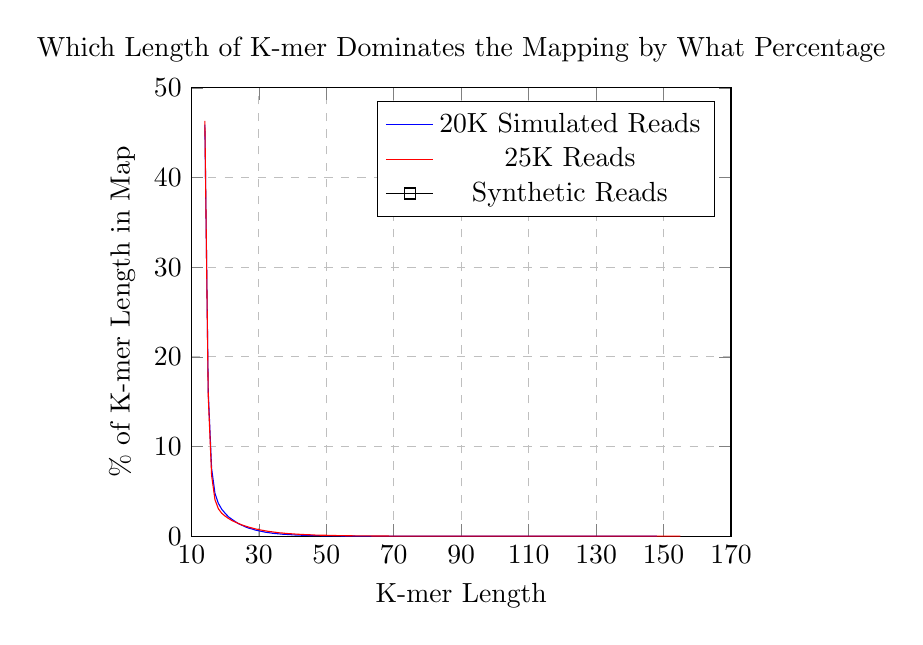
\begin{tikzpicture}
 	\begin{axis}[
 	title={Which Length of K-mer Dominates the Mapping by What Percentage},
 	xlabel={K-mer Length},
 	ylabel={\% of K-mer Length in Map  },
 	xmin=10, xmax=170,
 	ymin=0, ymax=50,
 	xtick={10,30,50,70,90,110,130,150,170},
 	ytick={0,10,20,30,40,50},
 	legend pos=north east,
 	ymajorgrids=true,
 	xmajorgrids=true,
 	grid style=dashed,
 	]
 	
 	\addplot[
 	color=blue,
 	mark=dot,
 	]
 	coordinates {
 		( 14 , 45.91 )( 15 , 16.12 )( 16 , 7.55 )( 17 , 4.77 )( 18 , 3.66 )( 19 , 3.01 )( 20 , 2.56 )( 21 , 2.16 )( 22 , 1.89 )( 23 , 1.63 )( 24 , 1.39 )( 25 , 1.22 )( 26 , 1.04 )( 27 , 0.9 )( 28 , 0.8 )( 29 , 0.68 )( 30 , 0.6 )( 31 , 0.52 )( 32 , 0.44 )( 33 , 0.39 )( 34 , 0.33 )( 35 , 0.29 )( 36 , 0.26 )( 37 , 0.22 )( 38 , 0.2 )( 39 , 0.18 )( 40 , 0.15 )( 41 , 0.13 )( 42 , 0.12 )( 43 , 0.1 )( 44 , 0.09 )( 45 , 0.08 )( 46 , 0.07 )( 47 , 0.06 )( 48 , 0.06 )( 49 , 0.05 )( 50 , 0.04 )( 51 , 0.04 )( 52 , 0.03 )( 53 , 0.03 )( 54 , 0.03 )( 55 , 0.02 )( 56 , 0.02 )( 57 , 0.02 )( 58 , 0.02 )( 59 , 0.01 )( 60 , 0.01 )( 61 , 0.01 )( 62 , 0.01 )( 63 , 0.01 )( 64 , 0.01 )( 65 , 0.01 )( 66 , 0.01 )( 67 , 0.01 )( 68 , 0.0 )( 69 , 0.0 )( 70 , 0.0 )( 71 , 0.0 )( 72 , 0.0 )( 73 , 0.0 )( 74 , 0.0 )( 75 , 0.0 )( 76 , 0.0 )( 77 , 0.0 )( 78 , 0.0 )( 79 , 0.0 )( 80 , 0.0 )( 81 , 0.0 )( 82 , 0.0 )( 83 , 0.0 )( 84 , 0.0 )( 85 , 0.0 )( 86 , 0.0 )( 87 , 0.0 )( 88 , 0.0 )( 89 , 0.0 )( 90 , 0.0 )( 91 , 0.0 )( 92 , 0.0 )( 93 , 0.0 )( 94 , 0.0 )( 95 , 0.0 )( 96 , 0.0 )( 97 , 0.0 )( 98 , 0.0 )( 99 , 0.0 )( 100 , 0.0 )( 101 , 0.0 )( 103 , 0.0 )( 104 , 0.0 )( 105 , 0.0 )( 108 , 0.0 )( 109 , 0.0 )( 111 , 0.0 )( 113 , 0.0 )( 116 , 0.0 )( 117 , 0.0 )( 122 , 0.0 )( 126 , 0.0 )( 127 , 0.0 )( 128 , 0.0 )( 129 , 0.0 )( 139 , 0.0 )( 140 , 0.0 )( 142 , 0.0 )( 148 , 0.0 )
 	};
 	\addlegendentry{20K Simulated Reads}
 	\addplot[
 	color=red,
 	mark=dot,
 	]
 	coordinates {
 		( 14 , 46.31 )( 15 , 15.69 )( 16 , 6.78 )( 17 , 4.06 )( 18 , 3.06 )( 19 , 2.56 )( 20 , 2.24 )( 21 , 1.98 )( 22 , 1.75 )( 23 , 1.58 )( 24 , 1.41 )( 25 , 1.25 )( 26 , 1.13 )( 27 , 1.01 )( 28 , 0.91 )( 29 , 0.81 )( 30 , 0.73 )( 31 , 0.66 )( 32 , 0.59 )( 33 , 0.53 )( 34 , 0.48 )( 35 , 0.43 )( 36 , 0.38 )( 37 , 0.35 )( 38 , 0.31 )( 39 , 0.28 )( 40 , 0.26 )( 41 , 0.23 )( 42 , 0.21 )( 43 , 0.19 )( 44 , 0.17 )( 45 , 0.16 )( 46 , 0.14 )( 47 , 0.12 )( 48 , 0.11 )( 49 , 0.1 )( 50 , 0.1 )( 51 , 0.09 )( 52 , 0.08 )( 53 , 0.07 )( 54 , 0.07 )( 55 , 0.06 )( 56 , 0.05 )( 57 , 0.05 )( 58 , 0.04 )( 59 , 0.04 )( 60 , 0.03 )( 61 , 0.03 )( 62 , 0.03 )( 63 , 0.03 )( 64 , 0.02 )( 65 , 0.02 )( 66 , 0.02 )( 67 , 0.02 )( 68 , 0.02 )( 69 , 0.01 )( 70 , 0.01 )( 71 , 0.01 )( 72 , 0.01 )( 73 , 0.01 )( 74 , 0.01 )( 75 , 0.01 )( 76 , 0.01 )( 77 , 0.01 )( 78 , 0.01 )( 79 , 0.01 )( 80 , 0.01 )( 81 , 0.0 )( 82 , 0.0 )( 83 , 0.0 )( 84 , 0.0 )( 85 , 0.0 )( 86 , 0.0 )( 87 , 0.0 )( 88 , 0.0 )( 89 , 0.0 )( 90 , 0.0 )( 91 , 0.0 )( 92 , 0.0 )( 93 , 0.0 )( 94 , 0.0 )( 95 , 0.0 )( 96 , 0.0 )( 97 , 0.0 )( 98 , 0.0 )( 99 , 0.0 )( 100 , 0.0 )( 101 , 0.0 )( 102 , 0.0 )( 103 , 0.0 )( 104 , 0.0 )( 105 , 0.0 )( 106 , 0.0 )( 107 , 0.0 )( 108 , 0.0 )( 109 , 0.0 )( 110 , 0.0 )( 111 , 0.0 )( 112 , 0.0 )( 113 , 0.0 )( 114 , 0.0 )( 115 , 0.0 )( 116 , 0.0 )( 117 , 0.0 )( 118 , 0.0 )( 119 , 0.0 )( 120 , 0.0 )( 121 , 0.0 )( 122 , 0.0 )( 123 , 0.0 )( 124 , 0.0 )( 125 , 0.0 )( 126 , 0.0 )( 127 , 0.0 )( 128 , 0.0 )( 129 , 0.0 )( 130 , 0.0 )( 131 , 0.0 )( 132 , 0.0 )( 133 , 0.0 )( 134 , 0.0 )( 135 , 0.0 )( 136 , 0.0 )( 137 , 0.0 )( 138 , 0.0 )( 141 , 0.0 )( 143 , 0.0 )( 144 , 0.0 )( 147 , 0.0 )( 148 , 0.0 )( 152 , 0.0 )( 155 , 0.0 )
 	};
 	\addlegendentry{25K Reads}
 	\addplot[
 	color=black,
 	mark=square,
 	]
 	coordinates {
 		( 10000 , 100.0 )
 	};
 	\addlegendentry{Synthetic Reads}
 	\end{axis}
 	\end{tikzpicture}
 	
 	
 	\caption{For Gradually Increasing the Length of K-mer in Naive FM-index Approach, Domination of Small K-mers is Clear In the Graph. Synthetic Reads has No Room in the Plot, Because It is Considered as Outliers. It Would be A Point at (10000, 100.0) as It has No Error.} \label{fig:statKmerLength}
 \end{figure}
 \begin{figure}
 	\centering
 	
 	
 	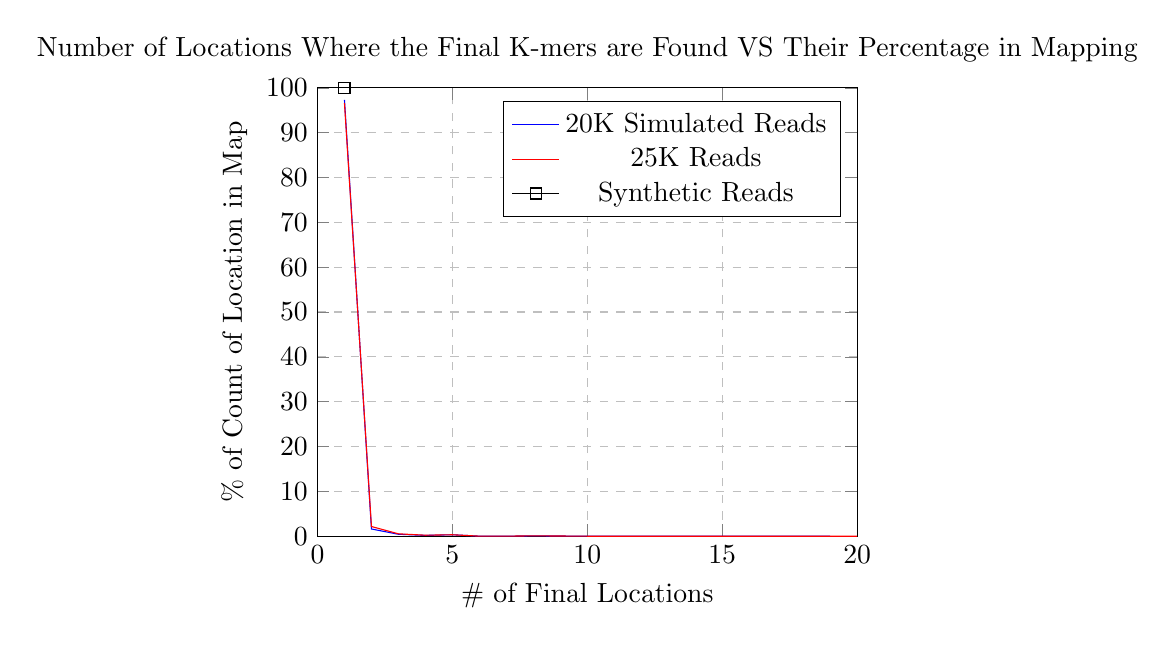
\begin{tikzpicture}
 	\begin{axis}[
 	title={Number of Locations Where the Final K-mers are Found VS Their Percentage in Mapping},
 	xlabel={\# of Final Locations},
 	ylabel={\% of Count of Location in Map  },
 	xmin=0, xmax=20,
 	ymin=0, ymax=100,
 	xtick={0,5,10,15,20},
 	ytick={0,10,20,30,40,50,60,70,80,90,100},
 	legend pos=north east,
 	ymajorgrids=true,
 	xmajorgrids=true,
 	grid style=dashed,
 	]
 	
 	\addplot[
 	color=blue,
 	mark=dot,
 	]
 	coordinates {
 		( 1 , 97.32 )( 2 , 1.61 )( 3 , 0.43 )( 4 , 0.18 )( 5 , 0.32 )( 6 , 0.01 )( 7 , 0.01 )( 8 , 0.07 )( 9 , 0.04 )( 10 , 0.0 )( 11 , 0.0 )( 12 , 0.0 )( 13 , 0.0 )( 14 , 0.0 )( 16 , 0.0 )( 17 , 0.0 )( 18 , 0.0 )( 19 , 0.0 )
 	};
 	\addlegendentry{20K Simulated Reads}
 	\addplot[
 	color=red,
 	mark=dot,
 	]
 	coordinates {
 		( 1 , 96.62 )( 2 , 2.16 )( 3 , 0.53 )( 4 , 0.22 )( 5 , 0.32 )( 6 , 0.01 )( 7 , 0.01 )( 8 , 0.08 )( 9 , 0.04 )( 10 , 0.0 )( 11 , 0.0 )( 12 , 0.0 )( 13 , 0.0 )( 14 , 0.0 )( 15 , 0.0 )( 16 , 0.0 )( 17 , 0.0 )( 18 , 0.0 )( 19 , 0.0 )( 20 , 0.0 )
 	};
 	\addlegendentry{25K Reads}
 	\addplot[
 	color=black,
 	mark=square,
 	]
 	coordinates {
 		( 1 , 100.0 )
 	};
 	\addlegendentry{Synthetic Reads}
 	\end{axis}
 	\end{tikzpicture}
 	
 	
 	\caption{Count of Final Locations and Their Percentage among the Whole Final Locations of K-mers.} \label{fig:statKmerLocation}
 \end{figure}
\end{document}